%% abtex2-modelo-trabalho-academico.tex, v-1.9.6 laurocesar
%% Copyright 2012-2016 by abnTeX2 group at http://www.abntex.net.br/ 
%%
%% This work may be distributed and/or modified under the
%% conditions of the LaTeX Project Public License, either version 1.3
%% of this license or (at your option) any later version.
%% The latest version of this license is in
%%   http://www.latex-project.org/lppl.txt
%% and version 1.3 or later is part of all distributions of LaTeX
%% version 2005/12/01 or later.
%%
%% This work has the L PPL maintenance status `maintained'.
%% 
%% The Current Maintainer of this work is the abnTeX2 team, led
%% by Lauro César Araujo. Further information are available on 
%% http://www.abntex.net.br/
%%
%% This work consists of the files abntex2-modelo-trabalho-academico.tex,
%% abntex2-modelo-include-comandos and abntex2-modelo-references.bib
% ------------------------------------------------------------------------
% ------------------------------------------------------------------------
% abnTeX2: Modelo de Trabalho Academico (tese de doutorado, dissertacao de
% mestrado e trabalhos monograficos em geral) em conformidade com 
% ABNT NBR 14724:2011: Informacao e documentacao - Trabalhos academicos -
% Apresentacao
% ------------------------------------------------------------------------
% ------------------------------------------------------------------------
% Personalização para o modelo Udesc 2024 9. ed. revisada e modificada
% Manual_13_05_2024_17175220258266_12510.pdf acesso em: 13/08/2024
% Autor: Felipe Joel Zimann (felipezimann@hotmail.com)
% Data: 02/12/2020 v1.0
% Data: 13/02/2021 v1.0.1 alterado tamanho numeração da página para 10pt
% Data: 13/08/2024 v1.0.2 alterado para citação (Autor, Ano) ao invés de (AUTOR, Ano) conforme ABNT NBR 10520:2023
% ------------------------------------------------------------------------
% ------------------------------------------------------------------------

\documentclass[
	12pt,					% tamanho da fonte
	openright,				% capítulos começam em pág ímpar (insere página vazia caso preciso)
	oneside,				% para impressão em recto e verso (twoside). Oposto a (oneside)
	a4paper,				% tamanho do papel. 
	chapter=TITLE,			% títulos de capítulos convertidos em letras maiúsculas
	section=TITLE,			% títulos de seções convertidos em letras maiúsculas
	sumario=abnt-6027-2012,
	english,				% idioma adicional para hifenização
	brazil,					% o último idioma é o principal do documento
	fleqn,					% equações alinhadas a esquerda (UDESC/CCT)+
	]{abntex2}

% ----------------------------------------------------------
% Pacotes básicos 
% ----------------------------------------------------------
\usepackage{amsmath}							% Pacote matemático
\usepackage{amssymb}							% Pacote matemático
\usepackage{amsfonts}							% Pacote matemático
%\usepackage{lmodern}							% Usa a fonte Latin Modern		
\usepackage{mathptmx} 							% Usa a fonte Times New Roman	 (UDESC/CCT)
\usepackage[T1]{fontenc}						% Selecao de codigos de fonte.
\usepackage[utf8]{inputenc}						% Codificacao do documento (conversão automática dos acentos)
\usepackage{lastpage}							% Usado pela Ficha catalográfica
\usepackage{indentfirst}						% Indenta o primeiro parágrafo de cada seção.
\usepackage[dvipsnames,table]{xcolor}			% Controle das cores
\usepackage{graphicx}							% Inclusão de gráficos
\usepackage{microtype} 							% para melhorias de justificação
\usepackage{lipsum}								% para geração de dummy text
\usepackage[brazilian,hyperpageref]{backref}	% Paginas com as citações na bibl
\usepackage[alf,abnt-emphasize=bf,abnt-full-initials=yes]{abntex2cite}					% Citações padrão ABNT
%\usepackage[num]{abntex2cite}					% Citações padrão ABNT numérica
\usepackage{adjustbox}							% Pacote de ajuste de boxes
\usepackage{subcaption}							% Inclusão de Subfiguras e sublegendas		
\usepackage{enumitem}							% Personalização de listas
\usepackage{siunitx}							% Grandezas e unidades
\usepackage[section]{placeins}					% Manter as figuras delimitadas na respectiva seção com a opção [section]
\usepackage{multirow}							% Multi colunas nas tabelas
\usepackage{array,tabularx} 					% Pacotes de tabelas
\usepackage{booktabs}							% Pacote de tabela profissonal
\usepackage{rotating}							% Rotacionar figuras e tabelas
\usepackage{xfrac}								% Fazer frações n/d em linha
\usepackage{bm}									% Negrito em modo matemático
\usepackage{xstring}							% Manipulação de strings
\usepackage{pgfplots}							% Pacote de Gráficos
\usepackage{tikz}								% Pacote de Figuras
\usepackage[american, cuteinductors,smartlabels, fulldiode, siunitx, americanvoltages, oldvoltagedirection, smartlabels]{circuitikz}						% Pacote de circuitos elétricos
\usepackage{chemformula}						% Pacote para fórmulas químicas
\usepackage{chngcntr}							% Pacte usado para deixar numeração de equações sequencial (UDESC/CCT)
\usepackage{amssymb} 							% Pacote matemático
\usepackage{pifont}							% Pacote de símbolos
\usepackage{makecell}							% Pacote de células de tabelas

\counterwithout{equation}{chapter}
% fonte: https://latex.org/forum/viewtopic.php?t=15392

% Comando para deixar numeração das equações contínua (1), (2), (3)... ao invés de organizar por capítulos (1.1)(1.2)... (2.1)(2.2)
%\renewcommand{\theequation}{\arabic{equation}}

%\numberwithin{equation}{section}


% Cabecalho cabeçalho somente com numeração de página 10pt
\makepagestyle{PagNumReduzida}
\makeevenhead{PagNumReduzida}{\ABNTEXfontereduzida\thepage}{}{}
\makeoddhead{PagNumReduzida}{}{}{\ABNTEXfontereduzida\thepage}
%fonte: https://github.com/abntex/abntex2/wiki/HowToCustomizarCabecalhoRodape
%fonte: Manual memoir seção 7.3 pg. 111 pdf http://linorg.usp.br/CTAN/macros/latex/contrib/memoir/memman.pdf 

% Personalização das opções das listas
\setlist[itemize]{leftmargin=\parindent}

% Citação online --- MODIFICAR ---
\newcommand{\citeshort}[1]{\citeauthoronline{#1}~(\citeyear{#1})}

\newcommand{\me}[1]{Elaborado pelo autor (#1).}

% Configuração do pgfplots
\pgfplotsset{compat=newest} %compat=1.14
\pgfplotsset{plot coordinates/math parser=false} 
\newlength\figureheight 
\newlength\figurewidth 

% Libraries do TiKz
\usetikzlibrary{quotes,angles,arrows}
\usetikzlibrary{through,calc,math}
\usetikzlibrary{graphs,backgrounds,fit}
\usetikzlibrary{shapes,positioning,patterns,shadows}
\usetikzlibrary{decorations.pathreplacing}
\usetikzlibrary{shapes.geometric}
\usetikzlibrary{arrows.meta}
\usetikzlibrary{external}

%\tikzexternalize[]
%\tikzexternalenable
%\tikzexternalize
%\tikzexternaldisable
%\tikzset{external/force remake}
%\tikzexternalize[shell escape=-enable-write18]

% Configurações do CircuiTiKz
\ctikzset{bipoles/thickness=1}
%\ctikzset{bipoles/length=1.2cm}
\ctikzset{monopoles/ground/width/.initial=.2}
\ctikzset{bipoles/resistor/height=0.25}
\ctikzset{bipoles/resistor/width=0.6}
\ctikzset{bipoles/capacitor/height=0.5}
\ctikzset{bipoles/capacitor/width=0.15}
\ctikzset{bipoles/generic/height=0.25}
\ctikzset{bipoles/generic/width=0.6}
%\ctikzset{bipoles/capacitor polar/length=0.5}
%\ctikzset{bipoles/diode/height=.375}
%\ctikzset{bipoles/diode/width=.3}
%\ctikzset{tripoles/thyristor/height=.8}
%\ctikzset{tripoles/thyristor/width=1}
\ctikzset{bipoles/vsourcesin/height=.5}
\ctikzset{bipoles/vsourcesin/width=.5}
\ctikzset{bipoles/cvsourceam/height=.6}
\ctikzset{bipoles/cvsourceam/width=.6}
%\ctikzset{tripoles/european controlled voltage source/width=.4}

\tikzstyle{every node}=[font=\footnotesize]
\tikzstyle{every path}=[line width=0.25pt,line cap=round,line join=round]
%\tikzstyle{every path}=[line cap=round,line join=round]


% Definição de cores MATLAB
\definecolor{matlab_blue}{rgb}	{         0,    0.4470,    0.7410}
\definecolor{matlab_orange}{rgb}{    0.8500,    0.3250,    0.0980}
\definecolor{matlab_yellow}{rgb}{    0.9290,    0.6940,    0.1250}
\definecolor{matlab_violet}{rgb}{    0.4940,    0.1840,    0.5560}
\definecolor{matlab_green}{rgb}	{	 0.4660,    0.6740,    0.1880}
\definecolor{matlab_lblue}{rgb}	{    0.3010,    0.7450,    0.9330}
\definecolor{matlab_red}{rgb}	{    0.6350,    0.0780,    0.1840}

% Personalização das legendas
\usepackage[format = plain, %hang
			justification = centering,
			labelsep = endash,
			singlelinecheck = false,
			skip = 6pt,
			listformat = simple]{caption}	

% Personalização das unidades
\sisetup{output-decimal-marker = {,}}
\sisetup{exponent-product = \cdot}
\sisetup{tight-spacing=true}
\sisetup{group-digits = false}

% Personalizações de tipo de colunas de tabelas
\newcolumntype{L}[1]{>{\raggedright\let\newline\\\arraybackslash\hspace{0pt}}m{#1}}
\newcolumntype{C}[1]{>{\centering\let\newline\\\arraybackslash\hspace{0pt}}m{#1}}
\newcolumntype{R}[1]{>{\raggedleft\let\newline\\\arraybackslash\hspace{0pt}}m{#1}}

% Personalizações de cores da UDESC
\definecolor{CapaAmareloUDESC}{RGB}{243,186,83}		% Especializacao
\definecolor{CapaVerdeUDESC}{RGB}{0,112,52}			% Mestrado
\definecolor{CapaVermelhoUDESC}{RGB}{171,35,21}		% Doutorado
\definecolor{CapaAzulUDESC}{RGB}{38,54,118} 		% Pós-Doutorado

% CONFIGURAÇÕES DE PACOTES
% Configurações do pacote backref
% Usado sem a opção hyperpageref de backref
\renewcommand{\backrefpagesname}{Citado na(s) página(s):~}
% Texto padrão antes do número das páginas
\renewcommand{\backref}{}
% Define os textos da citação
\renewcommand*{\backrefalt}[4]{
	\ifcase #1 %
	Nenhuma citação no texto.%
	\or
	Citado na página #2.%
	\else
	Citado #1 vezes nas páginas #2.%
	\fi}%

% alterando o aspecto da cor azul
%\definecolor{blue}{RGB}{41,5,195}

% informações do PDF
\makeatletter
\hypersetup{
	%pagebackref=true,
	pdftitle={\@title}, 
	pdfauthor={\@author},
	pdfsubject={\imprimirpreambulo},
	pdfcreator={LaTeX with abnTeX2},
	pdfkeywords={abnt}{latex}{abntex}{abntex2}{trabalho academico}, 
	colorlinks=true,       		% false: boxed links; true: colored links
	linkcolor=black,          	% color of internal links
	citecolor=black,        	% color of links to bibliography
	filecolor=black,      		% color of file links
	urlcolor=black,
	bookmarksdepth=4
}
\makeatother


\makeatletter
\newcommand{\includetikz}[1]{%
	\tikzsetnextfilename{#1}%
	\input{#1.tex}%
}
\makeatother


% ---
% Possibilita criação de Quadros e Lista de quadros.
% Ver https://github.com/abntex/abntex2/issues/176
%
\newcommand{\quadroname}{Quadro}
\newcommand{\listofquadrosname}{Lista de quadros}

\newfloat[chapter]{quadro}{loq}{\quadroname}
\newlistof{listofquadros}{loq}{\listofquadrosname}
\newlistentry{quadro}{loq}{0}

% configurações para atender às regras da ABNT
\setfloatadjustment{quadro}{\centering}
\counterwithout{quadro}{chapter}
\renewcommand{\cftquadroname}{\quadroname\space} 
\renewcommand*{\cftquadroaftersnum}{\hfill--\hfill}

\setfloatlocations{quadro}{hbtp} % Ver https://github.com/abntex/abntex2/issues/176
% ---


% Espaçamento depois do título
\setlength{\afterchapskip}{0.7\baselineskip}
% O tamanho do parágrafo é dado por:
\setlength{\parindent}{1.25cm}
% Controle do espaçamento entre um parágrafo e outro:
\setlength{\parskip}{0.0cm}  % tente também \onelineskip
%\SingleSpacing % Espaçamento simples 
\OnehalfSpacing % Espaçamento 1,5 (UDESC/CCT)
%\DoubleSpacing	% Espaçamento duplo

% ---
% Margens - NBR 14724/2011 - 5.1 Formato
% ---
\setlrmarginsandblock{3cm}{2cm}{*}
\setulmarginsandblock{3cm}{2cm}{*}
\checkandfixthelayout[fixed]
% ---


% To use externalize consider
%https://tex.stackexchange.com/questions/182783/tikzexternalize-not-compatible-with-miktex-2-9-abntex2-package
%Lauro Cesar digged into the problem until he came with a solution for me to test. And it Works!
%
%According to this link:
%
%The package calc changed the commands \setcounter and friends to be fragile. So you have to make them robust. The example below uses etoolbox with \robustify:
%
\usepackage{etoolbox}
\robustify\setcounter
\robustify\addtocounter
\robustify\setlength
\robustify\addtolength


%% How to silence memoir class warning against the use of caption package?
%% https://tex.stackexchange.com/questions/391993/how-to-silence-memoir-class-warning-against-the-use-of-caption-package
%\usepackage{silence}
%\WarningFilter*{memoir}{You are using the caption package with the memoir class}
%\WarningFilter*{Class memoir Warning}{You are using the caption package with the memoir class}

% --------------------------------------------------------
% INICIO DAS CUSTOMIZACOES PARA A UDESC
% --------------------------------------------------------

% --------------------------------------------------------
% Fontes padroes de part, chapter, section, subsection e subsubsection
% --------------------------------------------------------
% --- Chapter ---
\renewcommand{\ABNTEXchapterfont}{\fontseries{b}} %\bfseries
\renewcommand{\ABNTEXchapterfontsize}{\normalsize}
% --- Part ---
\renewcommand{\ABNTEXpartfont}{\ABNTEXchapterfont}
\renewcommand{\ABNTEXpartfontsize}{\LARGE}
% --- Section ---
\renewcommand{\ABNTEXsectionfont}{\normalfont}
\renewcommand{\ABNTEXsectionfontsize}{\normalsize}
% --- SubSection ---
\renewcommand{\ABNTEXsubsectionfont}{\fontseries{b}} %\bfseries
\renewcommand{\ABNTEXsubsectionfontsize}{\normalsize}
% --- SubSubSection ---
\renewcommand{\ABNTEXsubsubsectionfont}{\itshape}
\renewcommand{\ABNTEXsubsubsectionfontsize}{\normalsize}

\renewcommand{\ABNTEXsubsubsubsectionfont}{\normalfont}
\renewcommand{\ABNTEXsubsubsubsectionfontsize}{\normalsize}
% ---

% --------------------------------------------------------
% Fontes das entradas do sumario
% --------------------------------------------------------

\renewcommand{\cftpartfont}{\ABNTEXpartfont\selectfont}
\renewcommand{\cftpartpagefont}{\normalsize\selectfont}

\renewcommand{\cftchapterfont}{\ABNTEXchapterfont\selectfont}
\renewcommand{\cftchapterpagefont}{\normalsize\selectfont}

\renewcommand{\cftsectionfont}{\ABNTEXsectionfont\selectfont}
\renewcommand{\cftsectionpagefont}{\normalsize\selectfont}

\renewcommand{\cftsubsectionfont}{\ABNTEXsubsectionfont\selectfont}
\renewcommand{\cftsubsectionpagefont}{\normalsize\selectfont}

\renewcommand{\cftsubsubsectionfont}{\normalfont\itshape\selectfont}
\renewcommand{\cftsubsubsectionpagefont}{\normalsize\selectfont}

\renewcommand{\cftparagraphfont}{\normalfont\selectfont}
\renewcommand{\cftparagraphpagefont}{\normalsize\selectfont}

% --------------------------------------------------------
% Usando os pacotes hyperref, uppercase... 
% Para deixar a section do toc uppercase precisa de:
% --------------------------------------------------------
\usepackage{textcase}

\makeatletter

\let\oldcontentsline\contentsline
\def\contentsline#1#2{%
	\expandafter\ifx\csname l@#1\endcsname\l@section
	\expandafter\@firstoftwo
	\else
	\expandafter\@secondoftwo
	\fi
	{%
		\oldcontentsline{#1}{\MakeTextUppercase{#2}}%
	}{%
		\oldcontentsline{#1}{#2}%
	}%
}
\makeatother

% --------------------------------------------------------
% Renomenando as entradas de APÊNDICES E ANEXOS
% --------------------------------------------------------

\renewcommand{\apendicesname}{AP\^ENDICES}
\renewcommand{\anexosname}{ANEXOS}


% Manipulação de Strings
%\RequirePackage{xstring}

% Comando para inverter sobrenome e nome
\newcommand{\invertname}[1]{%
	\StrBehind{#1}{{}}, \StrBefore{#1}{{}}%
}%


% --------------------------------------------------------
% Alterando os estilos de Caption e Fonte
% --------------------------------------------------------
\makeatletter
% Define o comando \fonte que respeita as configurações de caption do memoir ou do caption
\renewcommand{\fonte}[2][\fontename]{%
	\M@gettitle{#2}%
	\memlegendinfo{#2}%
	\par
	\begingroup
	\@parboxrestore
	\if@minipage
	\@setminipage
	\fi
	\ABNTEXfontereduzida
	\configureseparator
	\captiondelim{\ABNTEXcaptionfontedelim}
	\@makecaption{#1}{\ignorespaces #2}\par
	\endgroup}


\captionstyle[\raggedright]{\raggedright}

\makeatother

\setlength{\cftbeforechapterskip}{0pt plus 0pt}
\renewcommand*{\insertchapterspace}{}

\newlength{\mylen}	% New length to use with spacing
\setlength{\mylen}{1pt}

\setlength{\cftbeforechapterskip}{\mylen}
\setlength{\cftbeforesectionskip}{\mylen}
\setlength{\cftbeforesubsectionskip}{\mylen}
\setlength{\cftbeforesubsubsectionskip}{\mylen}
\setlength{\cftbeforesubsubsubsectionskip}{\mylen}


% ---
% Ajuste das listas de abreviaturas e siglas ; e símbolos [Personalizada para UDESC com espaçamento 1,5]
% ---

% ---
% Redefinição da Lista de abreviaturas e siglas [Personalizada para UDESC com espaçamento 1,5]
\renewenvironment{siglas}{%
	\pretextualchapter{\listadesiglasname}
	\begin{symbols} 
		\setlength{\itemsep}{0pt}	% Ajuste para Espaçamento 1,5 (UDESC/CCT)
	}{% 
	\end{symbols}
	\cleardoublepage
}
% ---

% ---
% Redefinição da Lista de símbolos [Personalizada para UDESC com espaçamento 1,5]
\renewenvironment{simbolos}{%
	\pretextualchapter{\listadesimbolosname}
	\begin{symbols}
		\setlength{\itemsep}{0pt}	% Ajuste para Espaçamento 1,5 (UDESC/CCT)
	}{%
	\end{symbols}
	\cleardoublepage
}
% ---


% ---
% Remocao dos simbolos de < > das urls, ver manual pacote url pg 6 item 6
% https://github.com/abntex/biblatex-abnt/issues/16
\def\UrlLeft{}
\def\UrlRight{}
% ---

% ---
% FIM DAS CUSTOMIZACOES PARA A  Universidade do Estado de Santa Catarina - UDESC/CCT
% ---
	% Incliu pacotes básicos 

% -----------------------------------------------------------------
% Você pode adicionar seus pacotes a partir desta linha;
% -----------------------------------------------------------------

%\usepackage[showframe,pass]{geometry}
%\usepackage[11,12]{pagesel}

% -----------------------------------------------------------------
% Informações de dados para CAPA e FOLHA DE ROSTO
% -----------------------------------------------------------------
\titulo{INCLUSÃO E TECNOLOGIA: DESENVOLVIMENTO DE UMA FERRAMENTA DE AUXÍLIO PARA APLICAÇÕES MÓVEIS ACESSÍVEIS EM FLUTTER}%

\autor{Mateus Lucas Cruz Brandt}%
\orientador{Profa. Dra. Marília Guterres Ferreira}%

% ATENÇÃO: O símbolo {} indica o sobrenome para a ficha catalográfica.
% Exemplo: Sherlock Holmes {}da Silva para sobrenomes compostos;
% Exemplo: Arnold Alois {}Schwarzenegger para sobrenome simples.

\instituicao{Universidade do Estado de Santa Catarina, Centro de Ciências Tecnológicas, Programa de Pós--Graduação em Engenharia Elétrica}%

%\tipotrabalho{Tese (Doutorado)}
\tipotrabalho{Trabalho de Conclusão de Curso (Graduação)}

%\preambulo{Tese apresentada ao Programa de Pós--Graduação em Engenharia Elétrica do Centro de Ciências Tecnológicas da Universidade do Estado de Santa Catarina, como requisito parcial para a obtenção do grau de Doutor em Engenharia Elétrica.}

\preambulo{Trabalho de conclusão apresentado ao curso de Engenharia de Software do Centro de Educação Superior do Alto Vale do Itajaí (CEAVI), da Universidade do Estado de Santa Catarina (UDESC), como requisito parcial para obtenção do grau de bacharel em Engenharia de Software.}

\local{Rio do Sul}%

\data{\the\year}%
% ---

% compila o indice
\makeindex

% -----------------------------------------------------------------
% Início do documento
% -----------------------------------------------------------------
\begin{document}

\selectlanguage{brazil}
\frenchspacing  % Retira espaço extra obsoleto entre as frases.

% -----------------------------------------------------------------
% ELEMENTOS PRÉ-TEXTUAIS
% -----------------------------------------------------------------
\pretextual

% Você pode comentar os elementos que não deseja em seu trabalho;

% A capa pode ser escolhida dentro do arquivo Capa.tex (TCC, Master, Doc, ...)
% ---
% Capa
% ---


% --------------------------------------------------------
% Capa Padrão
% --------------------------------------------------------
\renewcommand{\imprimircapa}{%
	\begin{capa}%
		\center

		{\fontseries{b}\selectfont\MakeTextUppercase{UNIVERSIDADE DO ESTADO DE SANTA CATARINA -- UDESC}}
		
		{\fontseries{b}\selectfont\MakeTextUppercase{CENTRO DE EDUCAÇÃO SUPERIOR DO ALTO VALE DO ITAJAÍ -- CEAVI}}
		
		{\fontseries{b}\selectfont\MakeTextUppercase{ENGENHARIA DE SOFTWARE}}
		
		\vfill
		
		{\fontseries{b}\selectfont\MakeTextUppercase{\normalsize\imprimirautor}}
		
		\vfill
		\begin{center}
			{\fontseries{b}\selectfont\MakeTextUppercase{\imprimirtitulo}}
		\end{center}
		\vfill
		
		\vfill
		
		{\fontseries{b}\selectfont\MakeTextUppercase{\imprimirlocal}}
		\par
		{\fontseries{b}\selectfont \imprimirdata}
		\vspace*{1cm}
	\end{capa}
}



\imprimircapa				% Capa padrão
					% Elemento Obrigatório
% ---
% Folha de rosto
% ---








% --------------------------------------------------------
% folha de rosto 
% --------------------------------------------------------

\makeatletter

\renewcommand{\folhaderostocontent}{
	\begin{center}
		
		{\fontseries{b}\selectfont\MakeTextUppercase{\imprimirautor}}
		
		\vfill
		
		\begin{center}
			{\fontseries{b}\selectfont\MakeTextUppercase{\imprimirtitulo}}
		\end{center}
	
		\vspace*{1.5cm}

		\abntex@ifnotempty{\imprimirpreambulo}{%
			\hspace{.45\textwidth}
			{\begin{minipage}{.5\textwidth}
					\SingleSpacing
					\imprimirpreambulo\par
					\vspace*{4pt}
					{\imprimirorientadorRotulo~\imprimirorientador\par}
					\abntex@ifnotempty{\imprimircoorientador}{%
						{\imprimircoorientadorRotulo~\imprimircoorientador}%
					}%
			\end{minipage}}%
		}%
	
		
		\vfill
		
	{\fontseries{b}\selectfont\MakeTextUppercase{\imprimirlocal}}
	\par
	{\fontseries{b}\selectfont \imprimirdata}
	\vspace*{1cm}
	\end{center}
}


% (o * indica que haverá a ficha bibliográfica)
% ---
\imprimirfolhaderosto*
% ---


			% Elemento Obrigatório
% Caso não utilize a Ficha Catalográfica entre na folha de rosto e retire o * de dentro do arquivo FolhadeRosto

% ---
% Inserir a ficha bibliografica
% ---

% Isto é um exemplo de Ficha Catalográfica, ou ``Dados internacionais de
% catalogação-na-publicação''. Você pode utilizar este modelo como referência. 
% Porém, provavelmente a biblioteca da sua universidade lhe fornecerá um PDF
% com a ficha catalográfica definitiva após a defesa do trabalho. Quando estiver
% com o documento, salve-o como PDF no diretório do seu projeto e substitua todo
% o conteúdo de implementação deste arquivo pelo comando abaixo:



% \begin{fichacatalografica}
%     \includepdf{fig_ficha_catalografica.pdf}
% \end{fichacatalografica}


%	\setlength{\parindent}{0cm}
%	\setlength{\parskip}{0pt}
\begin{fichacatalografica}
	%\sffamily
	%\rmfamily
	%\ttfamily 
	\hbadness=10000
	\vspace*{\fill}					% Posição vertical
	\begin{center}					% Minipage Centralizado
	Para gerar a ficha catalográfica de teses e \\ 
	dissertações acessar o link:  \\
	https://www.udesc.br/bu/manuais/ficha
	
	\vspace*{8pt}
	
%	\begin{minipage}[c]{8cm}
%	\centering \sffamily
%	 Ficha catalográfica elaborada pelo(a) autor(a), com auxílio do programa de geração automática da Biblioteca Setorial do CCT/UDESC
%	\end{minipage}
	\fbox{\begin{minipage}[c]{13.5cm}		% Largura
	\flushright
	{\begin{minipage}[c]{10.5cm}		% Largura
	\vspace{1.25cm}
	%\footnotesize
	\setlength{\parindent}{1.5em}
	\noindent \invertname{\imprimirautor} \par
	\imprimirtitulo{ }/{ }\imprimirautor. -- \imprimirlocal, \imprimirdata .\par
	\pageref{LastPage} p. : il. \par
	\vspace{1.5em}
	\imprimirorientadorRotulo~\imprimirorientador.\par
	\imprimircoorientadorRotulo~\imprimircoorientador.\par
	\imprimirtipotrabalho~--~\imprimirinstituicao, \imprimirlocal, \imprimirdata.\par
	\vspace{1.5em}
		1. Palavra-chave.
		2. Palavra-chave.
		3. Palavra-chave.
 		4. Palavra-chave.
		5. Palavra-chave.
		I. \invertname{\imprimirorientador}.
		II. \invertname{\imprimircoorientador}.
		III. \imprimirinstituicao.
		IV. Título. %
	\vspace{1.25cm}	%		
	\end{minipage}%
	}% 
	\hspace{10mm}
	\end{minipage}}%
	
	\vspace*{0.5cm}
	
	\end{center}
\end{fichacatalografica}


%\begin{fichacatalografica}
%	\sffamily
%	\vspace*{\fill}					% Posição vertical
%	\begin{center}					% Minipage Centralizado
%	\fbox{\begin{minipage}[c][8cm]{13.5cm}		% Largura
%	\small
%	\imprimirautor
%	%Sobrenome, Nome do autor
%	
%	\hspace{0.5cm} \imprimirtitulo  / \imprimirautor. --
%	\imprimirlocal, \imprimirdata-
%	
%	\hspace{0.5cm} \pageref{LastPage} p. : il. (algumas color.) ; 30 cm.\\
%	
%	\hspace{0.5cm} \imprimirorientadorRotulo~\imprimirorientador\\
%	
%	\hspace{0.5cm}
%	\parbox[t]{\textwidth}{\imprimirtipotrabalho~--~\imprimirinstituicao,
%	\imprimirdata.}\\
%	
%	\hspace{0.5cm}
%		1. Palavra-chave1.
%		2. Palavra-chave2.
%		3. Palavra-chave3.
% 		4. Palavra-chave4.
%		5. Palavra-chave5.
%		I. Orientador.
%		II. Universidade xxx.
%		III. Faculdade de xxx.
%		IV. Título 			
%	\end{minipage}}
%	\end{center}
%\end{fichacatalografica}
% ---

	% Elemento Obrigatório (Verso da Folha)

% ---
% Inserir errata
% ---
\begin{errata}
Elemento opcional. 

Exemplo:

\vspace{\onelineskip}

Sobrenome, Prenome do Autor. Título de obra: subtítulo (se houver). Ano de depósito. Tipo do trabalho (grau e curso) - Vinculação acadêmica, local de apresentação/defesa, data.

\begin{table}[htb]
\center
\begin{tabular}{|p{2.4cm}|p{2cm}|p{3cm}|p{3cm}|}
  \hline
   \textbf{Folha} & \textbf{Linha}  & \textbf{Onde se lê}  & \textbf{Leia-se}  \\
    \hline
    1 & 10 & auto-conclavo & autoconclavo\\
   \hline
\end{tabular}
\end{table}

\end{errata}
% ---				% Elemento Opcional

% ---
% Inserir folha de aprovação
% ---

% Isto é um exemplo de Folha de aprovação, elemento obrigatório da NBR
% 14724/2011 (seção 4.2.1.3). Você pode utilizar este modelo até a aprovação
% do trabalho. Após isso, substitua todo o conteúdo deste arquivo por uma
% imagem da página assinada pela banca com o comando abaixo:
%
% \includepdf{folhadeaprovacao_final.pdf}
%
\begin{folhadeaprovacao}



	\begin{center}
		{\fontseries{b}\selectfont\MakeTextUppercase{\normalsize\imprimirautor}}
	\end{center}
    \vfill
    
	\vfill
	\begin{center}
		{\fontseries{b}\selectfont\MakeTextUppercase{\imprimirtitulo}}
	\end{center}
	\vfill

    
\abntex@ifnotempty{\imprimirpreambulo}{%
	\hspace{.45\textwidth}
	{\begin{minipage}{.5\textwidth}
			\SingleSpacing
			\imprimirpreambulo\par
			\vspace*{4pt}
			{\imprimirorientadorRotulo~\imprimirorientador\par}
			\abntex@ifnotempty{\imprimircoorientador}{%
				{\imprimircoorientadorRotulo~\imprimircoorientador}%
			}%
	\end{minipage}}%
}%


\vfill
        
	 \begin{center}
	 	
    	{\fontseries{b}\selectfont BANCA EXAMINADORA: }
    	\vspace*{1.75cm}
    
		Profa. Dra. Marília Guterres Ferreira \par
		CEAVI - UDESC
	 \end{center}
	
    {Membros:} 
    
	\begin{center}
		\vspace*{1.25cm}
		Mattheus da Hora França, Msc. \par
		CEAVI - UDESC
		
		\vspace*{1.25cm}
		Nome do Orientador e Titulação \par
		Nome da Instituição
	
	\end{center}
    
    \vspace*{\fill}  
    \begin{center}
    {\imprimirlocal, 05 de dezembro de \imprimirdata}
	\end{center}
    \vspace*{0.25cm}  
\end{folhadeaprovacao}
% ---




%\textbf{	{Orientador: \vspace{-16pt} }
%	\assinatura{\textbf{Prof. \imprimirorientador , Dr.} \\ Univ. XXX} 
%	{Coorientador: \vspace{-16pt}}   
%	\assinatura{\textbf{Prof. \imprimircoorientador , Dr.} \\ Univ. XXX}
%	
%	{Membros: \vspace{-16pt} } 
%	
%	% --- Exemplo de assinaturas em sequência ---       
%	\setlength{\ABNTEXsignwidth}{8.5cm}
%	
%	\assinatura{\textbf{Prof. Professor, Dr.} \\ Univ. XXX}
%	\assinatura{\textbf{Prof. Professor, Dr.} \\ Univ. XXX}
%	\assinatura{\textbf{Prof. Professor, Dr.} \\ Univ. XXX}
%	
%	% --- Exemplo de assinaturas lado a lado ---
%	\setlength{\ABNTEXsignwidth}{7.5cm}
	%
	%    \noindent\hfill\assinatura*{\textbf{Prof. Professor, Dr.} \\ Univ. XXX}%
	%    \hfill%
	%    \assinatura*{\textbf{Prof. Professor, Dr.} \\ Univ. XXX}%
	%    \hfill
	%    
	%    \noindent\hfill\assinatura*{\textbf{Prof. Professor, Dr.} \\ Univ. XXX}%
	%    \hfill%
	%    \assinatura*{\textbf{Prof. Professor, Dr.} \\ Univ. XXX}%
	%    \hfill}		% Elemento Obrigatório
% ---
% Dedicatória
% ---
\begin{dedicatoria}
   \vspace*{\fill}
%   \begin{flushright}
%   \noindent
%	Este trabalho é dedicado às crianças adultas que,\\
%	quando pequenas, sonharam em se tornar cientistas. 
%   \end{flushright}

{%
	\noindent\hspace{.5\textwidth}
	{\begin{minipage}{.5\textwidth}
			\begin{flushleft}
				Aos estudantes da Universidade do Estado de Santa Catarina, pela inspiração de sempre!
			\end{flushleft}
	\end{minipage}}%
\vspace*{3cm}
}%

\end{dedicatoria}
% ---
			% Elemento Opcional
% ---
% Agradecimentos
% ---
\begin{agradecimentos}

Gostaria de expressar minha profunda gratidão, em primeiro lugar, aos meus pais, que sempre foram minha base, me ensinando o valor do trabalho árduo e da dedicação.

À minha companheira, que esteve ao meu lado em todos os momentos, oferecendo apoio, incentivo e amor incondicional. Não tenho palavras suficientes para descrever o quanto sou grato por sua presença e por tudo que fez por mim, especialmente nos momentos mais difíceis.

Um agradecimento especial também ao Fedora, minha fiel companheira felina, cuja companhia trouxe leveza e observações silenciosas (mas julgadoras, como só um gato sabe fazer) durante o desenvolvimento deste trabalho.

Por fim, à minha orientadora, que desempenhou um papel essencial nesta jornada, guiando-me com paciência e incentivando-me a superar minhas próprias limitações. Seus elogios e orientações foram fundamentais para que eu acreditasse no meu potencial. Muito obrigado por tudo.

\end{agradecimentos}
% ---		% Elemento Opcional
% ---
% Epígrafe
% ---
\begin{epigrafe}
    \vspace*{\fill}
{%
	\noindent\hspace{.5\textwidth}
	{\begin{minipage}{.5\textwidth}
		\begin{flushright}
			“The only disability is when people cannot see human potential.” (DEBRA RUH)
		\end{flushright}
	\end{minipage}}%
	\vspace*{3cm}
}%
\end{epigrafe}
% ---				% Elemento Opcional
% ---
% RESUMOS
% ---

% resumo em português
\setlength{\absparsep}{18pt} % ajusta o espaçamento dos parágrafos do resumo
\begin{resumo}
Elemento obrigatório que contém a apresentação concisa dos pontos relevantes do trabalho, fornecendo uma visão rápida e clara do conteúdo e das conclusões do mesmo. A apresentação e a redação do resumo devem seguir os requisitos estipulados pela NBR 6028 (ABNT, 2003). Deve descrever de forma clara e sintética a natureza do trabalho, o objetivo, o método, os resultados e as conclusões, visando fornecer elementos para o leitor decidir sobre a consulta do trabalho no todo.

 \textbf{Palavras-chave}: Palavra 1. Palavra 2. Palavra 3. Palavra 4. Palavra 5.
\end{resumo}
				% Elemento Obrigatório
% ---
% Abstract
% ---

% resumo em inglês
\begin{resumo}[Abstract]
 \begin{otherlanguage*}{english}
   Elemento obrigatório para todos os trabalhos de conclusão de curso. Opcional para os demais trabalhos acadêmicos, inclusive para artigo científico. Constitui a versão do resumo em português para um idioma de divulgação internacional. Deve aparecer em página distinta e seguindo a mesma formatação do resumo em português.

   \textbf{Keywords}: Keyword 1. Keyword 2. Keyword 3. Keyword 4. Keyword 5.
 \end{otherlanguage*}
\end{resumo}
				% Elemento Obrigatório

% ---
% inserir lista de ilustrações
% ---
\pdfbookmark[0]{\listfigurename}{lof}
\listoffigures*
\cleardoublepage
% ---

% ---
% inserir lista de quadros
% ---
%\pdfbookmark[0]{\listofquadrosname}{loq}
%\listofquadros*
%\cleardoublepage
% ---


% ---
% inserir lista de tabelas
% ---
\pdfbookmark[0]{\listtablename}{lot}
\listoftables*
\cleardoublepage
% ---

% ---
% inserir lista de abreviaturas e siglas
% ---
\begin{siglas}
	\item[TCC] Trabalho de Conclusão de Curso
	\item[PCD] Pessoa com Deficiência
	\item[LBI] Lei Brasileira de Inclusão
\end{siglas}
% ---

% ---
% inserir lista de símbolos
% ---


\begin{simbolos}
  \item[@] Arroba
  \item[\%] Porcento
  \item[$^\circ$C] Graus Celsius
  \item[Ca] Cálcio
\end{simbolos}

% ---
				% Elemento Opcional
% ---
% inserir o sumario
% ---
\pdfbookmark[0]{\contentsname}{toc}
\tableofcontents*
\cleardoublepage
% ---
				% Elemento Obrigatório

% -----------------------------------------------------------------
% ELEMENTOS TEXTUAIS
% -----------------------------------------------------------------
\textual

\pagestyle{PagNumReduzida}						% Comando para cabeçalho somente com numeração de página 10pt
\aliaspagestyle{chapter}{PagNumReduzida}		% Deixar numeração da primeira página com tamanho igual ao resto da numeração
% ref.: https://groups.google.com/g/abntex2/c/CP7g8ZMgi-c/m/KjfEnn5b9a4J


% ---- Mantenha está estrutura, assim você deixa o trabalho mais organizado -------

%\chapter{Introdução}

\chapter{Introdução}

Este Trabalho de Conclusão de Curso (TCC) aborda o desenvolvimento de uma extensão Flutter que visa auxiliar os desenvolvedores no processo de criação de aplicações móveis acessíveis em Flutter. A motivação para este trabalho surge da crescente importância da inclusão e da acessibilidade no desenvolvimento de aplicações móveis, bem como da necessidade de simplificar e melhorar o processo de desenvolvimento de soluções acessíveis utilizando tecnologias modernas, como o Flutter.

O TCC foi desenvolvido seguindo uma metodologia baseada nas fases fundamentais da Engenharia de Software, incluindo análise (Engenharia de Requisitos), projeto, programação, testes e validação. Além disso, a execução do trabalho foi gerenciada utilizando a metodologia ágil, garantindo um desenvolvimento iterativo e incremental do projeto.

A introdução detalha o contexto, a problemática, os objetivos geral e específicos, a justificativa e a metodologia adotada no desenvolvimento do trabalho. Em seguida, o TCC é organizado em capítulos que abordam a revisão da literatura, o projeto e a implementação da extensão, os testes e a validação realizados com desenvolvedores e PCDs, e o gerenciamento do projeto. Por fim, as conclusões discutem os principais resultados, limitações e possíveis trabalhos futuros relacionados ao tema da acessibilidade em aplicações móveis.

\section{Problema}

A acessibilidade tem se tornado cada vez mais relevante no contexto do desenvolvimento de aplicações móveis, uma vez que possibilita a inclusão e a igualdade de oportunidades para pessoas com deficiência (PCDs). As aplicações móveis têm desempenhado um papel essencial no cotidiano das pessoas, e é imprescindível que elas sejam projetadas de forma inclusiva, garantindo uma experiência eficiente e satisfatória para todos os usuários. Neste cenário, o presente TCC se aplica ao desenvolvimento de aplicações móveis acessíveis utilizando o framework Flutter, que tem sido amplamente adotado devido à sua capacidade de criar aplicativos de alta qualidade e com desempenho otimizado para múltiplas plataforma. Contudo, o desenvolvimento de aplicações móveis acessíveis em Flutter ainda enfrenta desafios relacionados à complexidade e à necessidade de conhecimento especializado.

O problema abordado neste TCC é a dificuldade enfrentada pelos desenvolvedores ao implementar recursos de acessibilidade em aplicações móveis criadas com Flutter, em razão das lacunas de conhecimento e da complexidade inerente a essa tarefa. A solução proposta visa simplificar e tornar mais prática a criação de aplicações móveis acessíveis, contribuindo para a melhoria da experiência dos PCDs ao utilizar essas aplicações.

Para abordar este problema, serão investigadas as melhores práticas e técnicas disponíveis na literatura relacionadas à acessibilidade em aplicações móveis. Além disso, será desenvolvida uma aplicação de exemplo que demonstre a aplicabilidade das soluções propostas, servindo como referência para os desenvolvedores Flutter.

\subsection{Objetivo Geral}

O objetivo geral deste trabalho é apoiar o desenvolvimento de aplicativos móveis mais acessíveis. Para isso, visa-se criar uma extensão Flutter que facilite o processo de desenvolvimento de aplicações móveis acessíveis em Flutter para os desenvolvedores através da análise estática de código. A extensão fornecerá orientações e recomendações sobre a utilização de componentes e a aplicação de regras necessárias para cumprir com os requisitos de acessibilidade não funcionais. Através dessa abordagem, a extensão auxiliará os desenvolvedores a criar aplicativos mais inclusivos, melhorando a experiência dos PCDs ao utilizar essas aplicações.

Além disso, este trabalho visa aumentar a conscientização sobre a importância da acessibilidade no desenvolvimento de aplicações móveis. Para isso, serão publicados os requisitos de acessibilidade utilizados durante o desenvolvimento da extensão, a fim de promover uma compreensão mais ampla das melhores práticas e normas aplicáveis a essa área.

Dessa forma, a solução proposta contribui para resolver o problema apresentado ao facilitar a criação de aplicações móveis acessíveis em Flutter, fornecendo aos desenvolvedores as ferramentas e informações necessárias para atender aos requisitos de acessibilidade e, ao mesmo tempo, promovendo uma maior conscientização sobre a importância desse tema no contexto atual.

\subsection{Objetivos Específicos}

\subsubsection{Revisão da Literatura}

Realizar um mapeamentosistemático da literatura para identificar os requisitos não funcionais de acessibilidade necessários para aplicações móveis, permitindo estabelecer uma base sólida para o desenvolvimento da extensão proposta e garantir a aderência às melhores práticas e normas do campo.

\subsubsection{Projeto e Implementação da Extensão}

Desenvolver uma extensão Flutter que analise o código-fonte de aplicações móveis e forneça orientações e recomendações sobre a utilização de componentes e a aplicação de regras de acessibilidade. A extensão deverá ser integrada ao ambiente de desenvolvimento e ser capaz de identificar possíveis problemas de acessibilidade no código, sugerindo soluções e boas práticas para corrigi-los.

\subsubsection{Testes e Validação}

Realizar testes e validações da extensão com desenvolvedores e PCDs para avaliar a eficácia e a usabilidade da ferramenta. Os testes serão conduzidos em um ambiente controlado, permitindo identificar possíveis falhas e melhorias na extensão, bem como coletar feedbacks e sugestões para aprimorar a solução proposta.

\subsubsection{Documentar e Disseminar}

Documentar o processo de desenvolvimento da extensão, incluindo os requisitos de acessibilidade utilizados, as técnicas e as ferramentas empregadas, e os resultados obtidos. Além disso, disseminar os resultados do trabalho por meio de artigos, apresentações e publicações, a fim de promover a conscientização sobre a importância da acessibilidade no desenvolvimento de aplicações móveis.

\section{Justificativa}

Este TCC foi desenvolvido considerando a crescente importância da inclusão e acessibilidade no desenvolvimento de aplicações móveis, bem como a necessidade de simplificar e otimizar o processo de desenvolvimento de soluções acessíveis utilizando Flutter. A escolha do Flutter como tecnologia central deste trabalho se justifica por ser um framework em rápido crescimento, adotado por um número cada vez maior de desenvolvedores, devido à sua capacidade de criar aplicativos de alta qualidade e com desempenho otimizado para múltiplas plataforma. Ademais, o Flutter é mantido e promovido pelo Google, o que reforça sua relevância e potencial no cenário atual de desenvolvimento de aplicações móveis.

A escolha de uma extensão de análise estática de código como solução para o problema proposto se deve à sua capacidade de identificar problemas de acessibilidade no código-fonte e fornecer orientações e recomendações para corrigi-los. A análise estática de código é uma técnica amplamente utilizada no desenvolvimento de software para identificar possíveis falhas e melhorias no código, permitindo detectar problemas de acessibilidade em um estágio inicial do desenvolvimento e facilitar a correção desses problemas.

A justificativa para o desenvolvimento deste TCC, portanto, reside na combinação da importância de promover a acessibilidade e inclusão no desenvolvimento de aplicações móveis com a crescente adoção do Flutter como tecnologia de referência para o desenvolvimento de aplicativos. Ao criar uma extensão que facilite o desenvolvimento de aplicações móveis acessíveis em Flutter, este trabalho visa contribuir para a democratização da acessibilidade e a melhoria da experiência dos PCDs ao utilizar aplicações móveis.

\section{Metodologia}

A metodologia adotada neste TCC foi baseada nas fases fundamentais da Engenharia de Software, incluindo análise (Engenharia de Requisitos), projeto, programação, testes e validação. Além disso, a execução do trabalho foi gerenciada utilizando a metodologia ágil Scrum para garantir um desenvolvimento iterativo e incremental do projeto. A seguir, detalhamos cada uma das fases e ferramentas utilizadas na metodologia:

Engenharia de Requisitos: nesta fase, foi realizada um mapeamento sistemático da literatura para identificar os requisitos não funcionais de acessibilidade necessários para aplicações móveis. As principais fontes consultadas incluíram artigos científicos, livros e diretrizes de organizações especializadas em acessibilidade. As informações coletadas serviram como base para a definição dos requisitos que orientaram o desenvolvimento da extensão proposta.

Projeto: com os requisitos de acessibilidade definidos, a próxima etapa foi projetar a extensão para Flutter. Nesta fase, foram elaborados os diagramas e especificações técnicas necessárias para detalhar a arquitetura e o funcionamento da extensão, incluindo a definição das funcionalidades e a interação com o ambiente de desenvolvimento.

Programação: após a conclusão do projeto, a extensão foi implementada utilizando as linguagens de programação e as ferramentas compatíveis com o Flutter, como Dart, a extensão custom\_lint\_builder. O código-fonte foi versionado e gerenciado por meio do Git e hospedado em uma plataforma de repositórios (GitHub), para facilitar a colaboração e o acompanhamento das mudanças realizadas.

Testes e validação: a extensão desenvolvida foi submetida a uma série de testes, envolvendo desenvolvedores e PCDs, a fim de avaliar sua efetividade e garantir que os requisitos de acessibilidade fossem atendidos. Os testes foram realizados em diversas etapas do desenvolvimento e incluíram testes funcionais, de usabilidade e de acessibilidade. Além disso, os requisitos não funcionais coletados na revisão da literatura foram validados por meio de testes estáticos.

Gerenciamento do projeto (Scrum): para garantir um desenvolvimento eficiente e flexível, o projeto foi gerenciado utilizando a metodologia ágil Scrum. O trabalho foi dividido em Sprints, que são períodos de tempo fixos (geralmente de 2 a 4 semanas) nos quais um conjunto específico de tarefas é realizado. As tarefas foram organizadas e priorizadas em um Product Backlog.

\begin{figure}[!h]
	\centering
	\caption{Figura 1 - Modelo de metologia}
	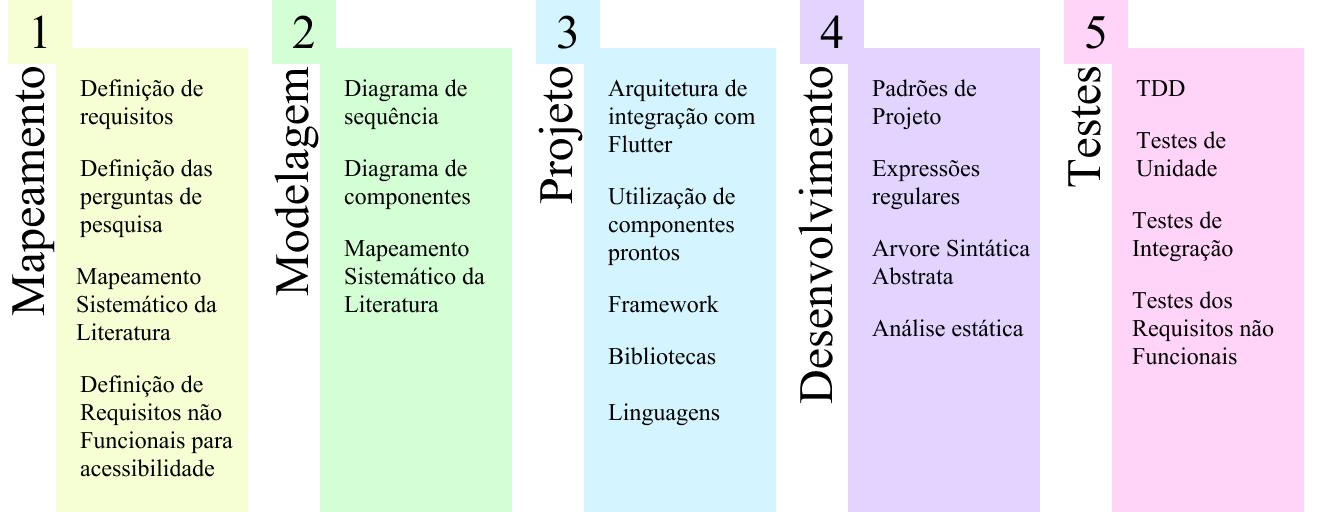
\includegraphics[scale=1]{Assets/Modelo de metodologia.png}
	\fonte{\me{2024}}
\end{figure}

A metodologia adotada permitiu um desenvolvimento estruturado e ágil do TCC, garantindo que a extensão proposta fosse construída de acordo com os requisitos de acessibilidade identificados. Além disso, a utilização do Scrum proporcionou flexibilidade e adaptabilidade durante o desenvolvimento, possibilitando ajustes e melhorias contínuas.

\section{Estrutura do trabalho}

O presente trabalho está organizado em capítulos que abordam os principais aspectos relacionados ao desenvolvimento da extensão proposta. A estrutura do trabalho é a seguinte:

\begin{itemize}
	\item Capítulo 2 - Revisão da Literatura: apresenta uma revisão da literatura sobre acessibilidade em aplicações móveis, abordando os principais conceitos, técnicas e ferramentas relacionadas ao tema.
	\item Capítulo 3 - Projeto e Implementação da Extensão: descreve o projeto e a implementação da extensão proposta, detalhando a arquitetura, as funcionalidades e as tecnologias utilizadas.
	\item Capítulo 4 - Testes e Validação: apresenta os testes e validações realizados com desenvolvedores e PCDs para avaliar a eficácia e a usabilidade da extensão.
	\item Capítulo 5 - Gerenciamento do Projeto: discute o gerenciamento do projeto, incluindo a metodologia ágil Scrum, as ferramentas utilizadas e os resultados obtidos.
	\item Capítulo 6 - Conclusões: apresenta as conclusões do trabalho, discutindo os principais resultados, limitações e possíveis trabalhos futuros relacionados ao tema da acessibilidade em aplicações móveis.
\end{itemize}

% -----------------------------------------------------------------
% ELEMENTOS PÓS-TEXTUAIS
% -----------------------------------------------------------------
\postextual

% Você pode comentar os elementos que não deseja em seu trabalho;

% Referências bibliográficas

%Notar que os autores continuam sendo transpostos em maiúsculas, como preconiza a ABNT NBR 6023:2002. 
%Se, no entanto, não desejar seguir esta regra,
%crie um novo arquivo .bst (por exemplo, novoestilo.bst)a partir do estilo
%usado (abntex2-cite-alf ou abntex2-cite-num) e retire todas as expressões
%"u" change.case$, lembrando-se de indicar o novo arquivo como estilo, por exemplo, 
%\bibliographystyle{novoestilo}, e colocar o arquivo criado na mesma
%pasta em que está compilando o documento.

% Arquivo alterado para citação (Autor, Ano) ao invés de (AUTOR, Ano) conforme ABNT NBR 10520:2023
\bibliographystyle{abntex2-alf_revNBR2023.bst}	

\bibliography{abntex2-ref_UDESC_2020}	% Elemento Obrigatório

% ----------------------------------------------------------
% Glossário
% ----------------------------------------------------------

%Consulte o manual da classe abntex2 para orientações sobre o glossário.

%\glossary

% ----------------------------------------------------------
% Glossário (Formatado Manualmente)
% ----------------------------------------------------------

\chapter*{GLOSSÁRIO}
\addcontentsline{toc}{chapter}{GLOSSÁRIO}

{ \setlength{\parindent}{0pt} % ambiente sem indentação

\textbf{Árvore Sintática Abstrata}: É uma representação abstrata (simplificada) da estrutura semântica de um código fonte escrito em uma certa linguagem de programação.

\textbf{Ánalise Estática}: Tem por objetivo encontrar vulnerabilidades e demais problemas na aplicação, e normalmente é executada durante a fase de revisão de código dentro do ciclo de vida de desenvolvimento de sistemas. Idealmente, tais ferramentas encontrariam falhas de segurança automaticamente e com alto grau de confiança.

\textbf{Framework}: É um conjunto de bibliotecas, APIs e ferramentas que auxiliam o desenvolvedor a criar aplicações de forma mais rápida e eficiente.

\textbf{pub.dev}: É o repositório oficial de pacotes Dart e Flutter, onde desenvolvedores podem publicar e compartilhar pacotes com a comunidade.

\textbf{LSP}: Language Server Protocol, é um protocolo de comunicação entre editores de código e servidores de linguagem que permite a execução de análises estáticas e outras funcionalidades de forma mais eficiente.

\textbf{Plugin}: É um componente de software que adiciona uma funcionalidade específica a um programa maior.

\textbf{Lint}: Lint é o termo de ciência da computação para uma ferramenta de análise de código estático usada para sinalizar erros de programação, bugs, erros estilísticos e construções suspeitas.

\textbf{Linter}: É uma ferramenta de análise estática que entrega o "Lint" para uma linguagem de programação específica.

} % fim ambiente sem indentação
				% Elemento Opcional

% ----------------------------------------------------------
% Apêndices
% ----------------------------------------------------------

% ---
% Inicia os apêndices
% ---
\begin{apendicesenv}

% Imprime uma página indicando o início dos apêndices
%\partapendices

% ----------------------------------------------------------
\chapter{TÍTULO}
% ----------------------------------------------------------


\end{apendicesenv}
% ---				% Elemento Opcional

% ----------------------------------------------------------
% Anexos
% ----------------------------------------------------------
%
% ---
% Inicia os anexos
% ---
\begin{anexosenv}

% Imprime uma página indicando o início dos anexos
%\partanexos

% ---
\chapter{TÍTULO}
% ---



\end{anexosenv}
				% Elemento Opcional

%%---------------------------------------------------------------------
%% INDICE REMISSIVO
%%---------------------------------------------------------------------

%\phantompart
%\printindex

%---------------------------------------------------------------------

%%---------------------------------------------------------------------
%% INDICE REMISSIVO (Formatado Manualmente)
%%---------------------------------------------------------------------

\chapter*{ÍNDICE}
\addcontentsline{toc}{chapter}{ÍNDICE}

{ \setlength{\parindent}{0pt}  % ambiente sem indentação
	
Andesito, 22, 50, 73

Argila, 52, 75, 121

Basalto, 25, 230, 235

	
	
	
	
} % fim ambiente sem indentação


		% Elemento Opcional



\end{document}

% -----------------------------------------------------------------
% Fim do Documento
% -----------------------------------------------------------------	